\documentclass[11pt, oneside, dvipdfmx]{book}
\newcommand{\folder}{/usr/local/share/texmf}
%Page setting
\setlength{\textwidth}{460pt}
\setlength{\topmargin}{-1truemm}
\setlength{\textheight}{650pt}
\setlength{\oddsidemargin}{-0.2truemm}
\setlength{\evensidemargin}{-0.2truemm}

%%%%%%%%%%%%
% 	 UsePackege	%
%%%%%%%%%%%%
\usepackage{amssymb}
\usepackage{amsmath}
\usepackage{amsthm}
\usepackage{ascmac}
\usepackage{lscape}
\usepackage{pifont}
\usepackage{cite}
\usepackage{ifthen}
\usepackage{framed}
\usepackage{mathrsfs}
\usepackage{booktabs}
\usepackage{algorithm}
\usepackage{algorithmic}
\usepackage{comment}
\usepackage{longtable}
% Font
%%%%%%%%%%%%%%
% 	Bold Number	%
%%%%%%%%%%%%%%
\newcommand{\bzero}{{\bf 0}}
\newcommand{\bone}{{\bf 1}}
%%%%%%%%%%%%%%
% 	Bold English	%
%%%%%%%%%%%%%%
% a
\newcommand{\ba}{{\mbox{\boldmath$a$}}}
\newcommand{\bA}{{\mbox{\boldmath$A$}}}
\newcommand{\sba}{{\mbox{\scriptsize\boldmath $a$}}}
% b
\newcommand{\bb}{{\mbox{\boldmath$b$}}}
\newcommand{\bB}{{\mbox{\boldmath$B$}}}
\newcommand{\sbb}{{\mbox{\scriptsize\boldmath $b$}}}
% c
\newcommand{\bc}{{\mbox{\boldmath$c$}}}
\newcommand{\bC}{{\mbox{\boldmath$C$}}}
\newcommand{\sbC}{{\mbox{\scriptsize\boldmath $C$}}}
\newcommand{\sbc}{{\mbox{\scriptsize\boldmath $c$}}}
% d
\newcommand{\bd}{{\mbox{\boldmath$d$}}}
\newcommand{\bD}{{\mbox{\boldmath$D$}}}
\newcommand{\sbd}{{\mbox{\scriptsize\boldmath $d$}}}
% e
\newcommand{\be}{{\mbox{\boldmath$e$}}}
\newcommand{\bE}{{\mbox{\boldmath$E$}}}
\newcommand{\sbe}{{\mbox{\scriptsize\boldmath $e$}}}
% f
\newcommand{\bbf}{{\mbox{\boldmath$f$}}}
\newcommand{\bF}{{\mbox{\boldmath$F$}}}
% g
\newcommand{\bg}{{\mbox{\boldmath$g$}}}
\newcommand{\bG}{{\mbox{\boldmath$G$}}}
% h
\newcommand{\bh}{{\mbox{\boldmath$h$}}}
\newcommand{\bH}{{\mbox{\boldmath$H$}}}
\newcommand{\sbH}{{\mbox{\scriptsize\boldmath$H$}}}
\newcommand{\sbh}{{\mbox{\scriptsize\boldmath$h$}}}
% i
\newcommand{\bi}{{\mbox{\boldmath$i$}}}
\newcommand{\sbi}{{\mbox{\scriptsize \boldmath$i$}}}
\newcommand{\bI}{{\mbox{\boldmath$I$}}}
% i
\newcommand{\bj}{{\mbox{\boldmath$j$}}}
\newcommand{\sbj}{{\mbox{\scriptsize \boldmath$j$}}}
\newcommand{\bJ}{{\mbox{\boldmath$J$}}}
% k
\newcommand{\bk}{{\mbox{\boldmath$k$}}}
\newcommand{\bK}{{\mbox{\boldmath$K$}}}
% l
%\newcommand{\ell}{{\mbox{\boldmath $l$}}}
\newcommand{\bl}{{\mbox{\boldmath$l$}}}
\newcommand{\bL}{{\mbox{\boldmath$L$}}}
% m
\newcommand{\bm}{{\mbox{\boldmath$m$}}}
\newcommand{\sbm}{{\mbox{\scriptsize \boldmath$m$}}}
\newcommand{\bM}{{\mbox{\boldmath$M$}}}
% n
\newcommand{\bn}{{\mbox{\boldmath$n$}}}
\newcommand{\bN}{{\mbox{\boldmath$N$}}}
\newcommand{\sbn}{{\mbox{\scriptsize \boldmath$n$}}}
\newcommand{\sbN}{{\mbox{\scriptsize\boldmath $N$}}}
% o
\newcommand{\bo}{{\mbox{\boldmath$o$}}}
\newcommand{\bO}{{\mbox{\boldmath$O$}}}
% p
\newcommand{\bp}{{\mbox{\boldmath$p$}}}
\newcommand{\bP}{{\mbox{\boldmath$P$}}}
\newcommand{\sbp}{{\mbox{\scriptsize \boldmath$p$}}}
% q
\newcommand{\bq}{{\mbox{\boldmath$q$}}}
\newcommand{\bQ}{{\mbox{\boldmath$Q$}}}
% r
\newcommand{\br}{{\mbox{\boldmath$r$}}}
\newcommand{\bR}{{\mbox{\boldmath$R$}}}
\newcommand{\sbr}{{\mbox{\scriptsize\boldmath$r$}}}
% s
\newcommand{\bs}{{\mbox{\boldmath$s$}}}
\newcommand{\sbs}{{\mbox{\scriptsize \boldmath$s$}}}
\newcommand{\bS}{{\mbox{\boldmath$S$}}}
% t
\newcommand{\bt}{{\mbox{\boldmath$t$}}}
\newcommand{\bT}{{\mbox{\boldmath$T$}}}
% u
\newcommand{\bu}{{\mbox{\boldmath$u$}}}
\newcommand{\bU}{{\mbox{\boldmath$U$}}}
\newcommand{\sbu}{{\mbox{\scriptsize\boldmath $u$}}}
% v
\newcommand{\bv}{{\mbox{\boldmath$v$}}}
\newcommand{\bV}{{\mbox{\boldmath$V$}}}
% w
\newcommand{\bw}{{\mbox{\boldmath$w$}}}
\newcommand{\bW}{{\mbox{\boldmath$W$}}}
\newcommand{\sbW}{{\mbox{\scriptsize\boldmath $W$}}}
\newcommand{\sbw}{{\mbox{\scriptsize\boldmath $w$}}}
% x
\newcommand{\bx}{{\mbox{\boldmath$x$}}}
\newcommand{\bX}{{\mbox{\boldmath$X$}}}
\newcommand{\sbx}{{\mbox{\scriptsize\boldmath $x$}}}
\newcommand{\sbX}{{\mbox{\scriptsize\boldmath $X$}}}
%y
\newcommand{\by}{{\mbox{\boldmath$y$}}}
\newcommand{\bY}{{\mbox{\boldmath$Y$}}}
\newcommand{\sby}{{\mbox{\scriptsize\boldmath $y$}}}
\newcommand{\sbY}{{\mbox{\scriptsize\boldmath $Y$}}}
%z
\newcommand{\bz}{{\mbox{\boldmath$z$}}}
\newcommand{\bZ}{{\mbox{\boldmath$Z$}}}
\newcommand{\sbz}{{\mbox{\scriptsize\boldmath$z$}}}
\newcommand{\sbZ}{{\mbox{\scriptsize\boldmath$Z$}}}


%%%%%%%%%%%
% 	Bold Grik	%
%%%%%%%%%%%
% alpha
\newcommand{\balpha}{{\mbox{\boldmath$\alpha$}}}
\newcommand{\sbalpha}{{\mbox{\scriptsize\boldmath$\alpha$}}}
% beta
\newcommand{\bbeta}{{\mbox{\boldmath$\beta$}}}
\newcommand{\sbbeta}{{\mbox{\scriptsize\boldmath$\beta$}}}
% gamma
\newcommand{\bgamma}{{\mbox{\boldmath$\gamma$}}}
\newcommand{\bGamma}{{\mbox{\boldmath$\Gamma$}}}
\newcommand{\sbgamma}{{\mbox{\scriptsize\boldmath$\gamma$}}}
% delta
\newcommand{\bdelta}{{\mbox{\boldmath$\delta$}}}
\newcommand{\bDelta}{{\mbox{\boldmath$\Delta$}}}
\newcommand{\sbdelta}{{\mbox{\scriptsize\boldmath$\delta$}}}
% epsilon
\newcommand{\bepsilon}{{\mbox{\boldmath$\epsilon$}}}
\newcommand{\bvarepsilon}{{\mbox{\boldmath$\varepsilon$}}}
\newcommand{\sbvarepsilon}{{\mbox{\scriptsize\boldmath$\varepsilon$}}}
% zeta
\newcommand{\bzeta}{{\mbox{\boldmath$\zeta$}}}
% eta
\newcommand{\etab}{{\mbox{\boldmath$\eta$}}}
% theta
\newcommand{\btheta}{{\mbox{\boldmath$\theta$}}}
\newcommand{\bTheta}{{\mbox{\boldmath$\Theta$}}}
\newcommand{\bvartheta}{{\mbox{\boldmath$\vartheta$}}}
% iota
\newcommand{\biota}{{\mbox{\boldmath$\iota$}}}
\newcommand{\sbiota}{{\mbox{\scriptsize\boldmath$\iota$}}}
% kappa
\newcommand{\bkappa}{{\mbox{\boldmath$\kappa$}}}
% lambda
\newcommand{\blambda}{{\mbox{\boldmath$\lambda$}}}
\newcommand{\bLambda}{{\mbox{\boldmath$\Lambda$}}}
% mu
\newcommand{\bmu}{{\mbox{\boldmath$\mu$}}}
\newcommand{\sbmu}{{\mbox{\scriptsize\boldmath$\mu$}}}
% nu
\newcommand{\bnu}{{\mbox{\boldmath$\nu$}}}
\newcommand{\sbnu}{{\mbox{\scriptsize\boldmath$\nu$}}}
% xi
\newcommand{\bxi}{{\mbox{\boldmath$\xi$}}}
\newcommand{\bXi}{{\mbox{\boldmath$\Xi$}}}
% pi
\newcommand{\bpi}{{\mbox{\boldmath$\pi$}}}
\newcommand{\bPi}{{\mbox{\boldmath$\Pi$}}}
\newcommand{\bvarpi}{{\mbox{\boldmath$\varpi$}}}
% rho
\newcommand{\brho}{{\mbox{\boldmath$\rho$}}}
\newcommand{\bvarrho}{{\mbox{\boldmath$\varrho$}}}
% sigma
\newcommand{\bsigma}{{\mbox{\boldmath$\sigma$}}}
\newcommand{\bSigma}{{\mbox{\boldmath$\Sigma$}}}
\newcommand{\bvarsigma}{{\mbox{\boldmath$\varsigma$}}}
% tau
\newcommand{\btau}{{\mbox{\boldmath$\tau$}}}
% upsilon
\newcommand{\bupsilon}{{\mbox{\boldmath$\upsilon$}}}
\newcommand{\bUpsilon}{{\mbox{\boldmath$\Upsilon$}}}
% phi
\newcommand{\bphi}{{\mbox{\boldmath$\phi$}}}
\newcommand{\bPhi}{\mathbf \Phi}
\newcommand{\bvarphi}{{\mbox{\boldmath$\varphi$}}}
% chi
\newcommand{\bchi}{{\mbox{\boldmath$\chi$}}}
% psi
\newcommand{\bpsi}{{\mbox{\boldmath$\psi$}}}
\newcommand{\bPsi}{\mathbf \Psi}
% omega
\newcommand{\bomega}{{\mbox{\boldmath$\omega$}}}
\newcommand{\bOmega}{{\mbox{\boldmath$\Omega$}}}
% nabla
\newcommand{\bnabla}{{\mbox{\boldmath$\nabla$}}}

% calligraphic letters
\newcommand{\cA}{{\cal A}}
\newcommand{\cB}{{\cal B}}
\newcommand{\cC}{{\cal C}}
\newcommand{\cD}{{\cal D}}
\newcommand{\cE}{{\cal E}}
\newcommand{\cF}{{\cal F}}
\newcommand{\cG}{{\cal G}}
\newcommand{\cH}{{\cal H}}
\newcommand{\cI}{{\cal I}}
\newcommand{\cJ}{{\cal J}}
\newcommand{\cK}{{\cal K}}
\newcommand{\cL}{{\cal L}}
\newcommand{\cM}{{\cal M}}
\newcommand{\cN}{{\cal N}}
\newcommand{\cO}{{\cal O}}
\newcommand{\cP}{{\cal P}}
\newcommand{\cQ}{{\cal Q}}
\newcommand{\cR}{{\cal R}}
\newcommand{\cS}{{\cal S}}
\newcommand{\cT}{{\cal T}}
\newcommand{\cU}{{\cal U}}
\newcommand{\cV}{{\cal V}}
\newcommand{\cW}{{\cal W}}
\newcommand{\cX}{{\cal X}}
\newcommand{\cY}{{\cal Y}}
\newcommand{\cZ}{{\cal Z}}
% calligraphic letters
\newcommand{\mA}{{\mathscr A}}
\newcommand{\mB}{{\mathscr B}}
\newcommand{\mC}{{\mathscr C}}
\newcommand{\mD}{{\mathscr D}}
\newcommand{\mE}{{\mathscr E}}
\newcommand{\mF}{{\mathscr F}}
\newcommand{\mG}{{\mathscr G}}
\newcommand{\mH}{{\mathscr H}}
\newcommand{\mI}{{\mathscr I}}
\newcommand{\mJ}{{\mathscr J}}
\newcommand{\mK}{{\mathscr K}}
\newcommand{\mL}{{\mathscr L}}
\newcommand{\mM}{{\mathscr M}}
\newcommand{\mN}{{\mathscr N}}
\newcommand{\mO}{{\mathscr O}}
\newcommand{\mP}{{\mathscr P}}
\newcommand{\mQ}{{\mathscr Q}}
\newcommand{\mR}{{\mathscr R}}
\newcommand{\mS}{{\mathscr S}}
\newcommand{\mT}{{\mathscr T}}
\newcommand{\mU}{{\mathscr U}}
\newcommand{\mV}{{\mathscr V}}
\newcommand{\mW}{{\mathscr W}}
\newcommand{\mX}{{\mathscr X}}
\newcommand{\mY}{{\mathscr Y}}
\newcommand{\mZ}{{\mathscr Z}}
% calligraphic letters
\newcommand{\bbA}{{\mathbb A}}
\newcommand{\bbB}{{\mathbb B}}
\newcommand{\bbC}{\mathbb{C}}
\newcommand{\bbD}{\mathbb{D}}
\newcommand{\bbE}{{\mathbb E}}
\newcommand{\bbF}{{\mathbb F}}
\newcommand{\bbG}{{\mathbb G}}
\newcommand{\bbH}{{\mathbb H}}
\newcommand{\bbI}{{\mathbb I}}
\newcommand{\bbJ}{{\mathbb J}}
\newcommand{\bbK}{{\mathbb K}}
\newcommand{\bbL}{\mathbb{L}}
\newcommand{\bbM}{{\mathbb M}}
\newcommand{\bbN}{\mathbb{N}}
\newcommand{\bbO}{{\mathbb O}}
\newcommand{\bbP}{\mathbb{P}}
\newcommand{\bbQ}{{\mathbb Q}}
\newcommand{\bbR}{\mathbb{R}}
\newcommand{\bbS}{\mathbb{S}}
\newcommand{\bbT}{{\mathbb T}}
\newcommand{\bbU}{{\mathbb U}}
\newcommand{\bbV}{\mathbb{V}}
\newcommand{\bbW}{{\mathbb W}}
\newcommand{\bbX}{\mathbb{X}}
\newcommand{\bbY}{\mathbb{Y}}
\newcommand{\bbZ}{{\mathbb Z}}
%%%%%%%%%%%%%%
% 	Tilde English	%
%%%%%%%%%%%%%%
% a
\newcommand{\tila}{\tilde{a}}
\newcommand{\tilA}{\tilde{A}}
% b
\newcommand{\tilb}{\tilde{b}}
\newcommand{\tilB}{\tilde{B}}
% c
\newcommand{\tilc}{\tilde{c}}
\newcommand{\tilC}{\tilde{C}}
% d
\newcommand{\tild}{\tilde{d}}
\newcommand{\tilD}{\tilde{D}}
% e
\newcommand{\tile}{\tilde{e}}
\newcommand{\tilE}{\tilde{E}}
% f
\newcommand{\tilf}{\tilde{f}}
\newcommand{\tilF}{\tilde{F}}
% g
\newcommand{\tilg}{\tilde{g}}
\newcommand{\tilG}{\tilde{G}}
% h
\newcommand{\tilh}{\tilde{h}}
\newcommand{\tilbh}{\tilde\bh}
\newcommand{\tilH}{\tilde{H}}
% i
\newcommand{\tili}{\tilde{i}}
\newcommand{\tilI}{\tilde{I}}
% i
\newcommand{\tilj}{\tilde{j}}
\newcommand{\tilJ}{\tilde{J}}
% k
\newcommand{\tilk}{\tilde{k}}
\newcommand{\tilK}{\tilde{K}}
% l
\newcommand{\till}{\tilde{l}}
\newcommand{\tilL}{\tilde{L}}
% m
\newcommand{\tilm}{\tilde{m}}
\newcommand{\tilM}{\tilde{M}}
% n
\newcommand{\tiln}{\tilde{n}}
\newcommand{\tilN}{\tilde{N}}
% o
\newcommand{\tilo}{\tilde{o}}
\newcommand{\tilO}{\tilde{O}}
% p
\newcommand{\tilp}{\tilde{p}}
\newcommand{\tilP}{\tilde{P}}
% q
\newcommand{\tilq}{\tilde{q}}
\newcommand{\tilQ}{\tilde{Q}}
\newcommand{\tilbq}{\tilde{\bq}}
% r
\newcommand{\tilr}{\tilde{r}}
\newcommand{\tilR}{\tilde{R}}
\newcommand{\tilcR}{\tilde{\cR}}
\newcommand{\tilbr}{\tilde{\br}}
% s
\newcommand{\tils}{\tilde{s}}
\newcommand{\tilS}{\tilde{S}}
% t
\newcommand{\tilt}{\tilde{t}}
\newcommand{\tilT}{\tilde{T}}
% u
\newcommand{\tilu}{\tilde{u}}
\newcommand{\tilU}{\tilde{U}}
% v
\newcommand{\tilv}{\tilde{v}}
\newcommand{\tilV}{\tilde{V}}
% w
\newcommand{\tilw}{\tilde{w}}
\newcommand{\tilW}{\tilde{W}}
% x
\newcommand{\tilx}{\tilde{x}}
\newcommand{\tilbx}{\tilde{\bx}}
\newcommand{\tilX}{\tilde{X}}
\newcommand{\tilbX}{\tilde{\bX}}
%y
\newcommand{\tily}{\tilde{y}}
\newcommand{\tilY}{\tilde{Y}}
\newcommand{\tilby}{\tilde{\by}}
\newcommand{\tilbY}{\tilde{\bY}}
%z
\newcommand{\tilz}{\tilde{z}}
\newcommand{\tilZ}{\tilde{Z}}
\newcommand{\tilbZ}{\tilde{\bZ}}


%%%%%%%%%%%%
%% 	Bold Grik	%
%%%%%%%%%%%%
%% alpha
\newcommand{\tilalpha}{\tilde{\alpha}}
%\newcommand{\sbalpha}{{\mbox{\scriptsize\boldmath$\alpha$}}}
%% beta
\newcommand{\tilbeta}{{\tilde{\beta}}}
%\newcommand{\sbbeta}{{\mbox{\scriptsize\boldmath$\beta$}}}
%% gamma
\newcommand{\tilgamma}{{\tilde{\gamma}}}
%\newcommand{\bGamma}{{\mbox{\boldmath$\Gamma$}}}
%\newcommand{\sbgamma}{{\mbox{\scriptsize\boldmath$\gamma$}}}
%% delta
%\newcommand{\bdelta}{{\mbox{\boldmath$\delta$}}}
%\newcommand{\bDelta}{{\mbox{\boldmath$\Delta$}}}
%\newcommand{\sbdelta}{{\mbox{\scriptsize\boldmath$\delta$}}}
%% epsilon
%\newcommand{\bepsilon}{{\mbox{\boldmath$\epsilon$}}}
%\newcommand{\bvarepsilon}{{\mbox{\boldmath$\varepsilon$}}}
%\newcommand{\sbvarepsilon}{{\mbox{\scriptsize\boldmath$\varepsilon$}}}
%% zeta
%\newcommand{\bzeta}{{\mbox{\boldmath$\zeta$}}}
%% eta
%\newcommand{\etab}{{\mbox{\boldmath$\eta$}}}
%% theta
%\newcommand{\btheta}{{\mbox{\boldmath$\theta$}}}
%\newcommand{\bTheta}{{\mbox{\boldmath$\Theta$}}}
%\newcommand{\bvartheta}{{\mbox{\boldmath$\vartheta$}}}
%% iota
%\newcommand{\biota}{{\mbox{\boldmath$\iota$}}}
%\newcommand{\sbiota}{{\mbox{\scriptsize\boldmath$\iota$}}}
%% kappa
%\newcommand{\bkappa}{{\mbox{\boldmath$\kappa$}}}
%% lambda
%\newcommand{\blambda}{{\mbox{\boldmath$\lambda$}}}
%\newcommand{\bLambda}{{\mbox{\boldmath$\Lambda$}}}
%% mu
%\newcommand{\bmu}{{\mbox{\boldmath$\mu$}}}
%\newcommand{\sbmu}{{\mbox{\scriptsize\boldmath$\mu$}}}
%% nu
%\newcommand{\bnu}{{\mbox{\boldmath$\nu$}}}
%\newcommand{\sbnu}{{\mbox{\scriptsize\boldmath$\nu$}}}
%% xi
%\newcommand{\bxi}{{\mbox{\boldmath$\xi$}}}
%\newcommand{\bXi}{{\mbox{\boldmath$\Xi$}}}
%% pi
%\newcommand{\bpi}{{\mbox{\boldmath$\pi$}}}
%\newcommand{\bPi}{{\mbox{\boldmath$\Pi$}}}
%\newcommand{\bvarpi}{{\mbox{\boldmath$\varpi$}}}
%% rho
%\newcommand{\brho}{{\mbox{\boldmath$\rho$}}}
%\newcommand{\bvarrho}{{\mbox{\boldmath$\varrho$}}}
%% sigma
%\newcommand{\bsigma}{{\mbox{\boldmath$\sigma$}}}
%\newcommand{\bSigma}{{\mbox{\boldmath$\Sigma$}}}
%\newcommand{\bvarsigma}{{\mbox{\boldmath$\varsigma$}}}
% tau
\newcommand{\tiltau}{{\mbox{$\tilde{\tau}$}}}
%% upsilon
%\newcommand{\bupsilon}{{\mbox{\boldmath$\upsilon$}}}
%\newcommand{\bUpsilon}{{\mbox{\boldmath$\Upsilon$}}}
%% phi
%\newcommand{\bphi}{{\mbox{\boldmath$\phi$}}}
%\newcommand{\bPhi}{\mathbf \Phi}
%\newcommand{\bvarphi}{{\mbox{\boldmath$\varphi$}}}
%% chi
%\newcommand{\bchi}{{\mbox{\boldmath$\chi$}}}
%% psi
%\newcommand{\bpsi}{{\mbox{\boldmath$\psi$}}}
%\newcommand{\bPsi}{\mathbf \Psi}
%% omega
%\newcommand{\bomega}{{\mbox{\boldmath$\omega$}}}
%\newcommand{\bOmega}{{\mbox{\boldmath$\Omega$}}}

%%%%%%%%%%%%%%
% 	Tilde English	%
%%%%%%%%%%%%%%
% a
\newcommand{\bara}{\bar{a}}
\newcommand{\barA}{\bar{A}}
% b
\newcommand{\barb}{\bar{b}}
\newcommand{\barB}{\bar{B}}
% c
\newcommand{\barc}{\bar{c}}
\newcommand{\barC}{\bar{C}}
% d
\newcommand{\bard}{\bar{d}}
\newcommand{\barD}{\bar{D}}
% e
\newcommand{\bare}{\bar{e}}
\newcommand{\barE}{\bar{E}}
% f
\newcommand{\barbf}{\bar{f}}
\newcommand{\barF}{\bar{F}}
% g
\newcommand{\barg}{\bar{g}}
\newcommand{\barG}{\bar{G}}
% h
\newcommand{\barh}{\bar{h}}
\newcommand{\barbh}{\bar\bh}
\newcommand{\barH}{\bar{H}}
% i
\newcommand{\bari}{\bar{i}}
\newcommand{\barI}{\bar{I}}
% i
\newcommand{\barj}{\bar{j}}
\newcommand{\barJ}{\bar{J}}
% k
\newcommand{\bark}{\bar{k}}
\newcommand{\barK}{\bar{K}}
% l
\newcommand{\barl}{\bar{l}}
\newcommand{\barL}{\bar{L}}
% m
\newcommand{\barm}{\bar{m}}
\newcommand{\barM}{\bar{M}}
% n
\newcommand{\barn}{\bar{n}}
\newcommand{\barN}{\bar{N}}
% o
\newcommand{\baro}{\bar{o}}
\newcommand{\barO}{\bar{O}}
% p
\newcommand{\barp}{\bar{p}}
\newcommand{\barP}{\bar{P}}
% q
\newcommand{\barq}{\bar{q}}
\newcommand{\barQ}{\bar{Q}}
% r
\newcommand{\barr}{\bar{r}}
\newcommand{\barR}{\bar{R}}
% s
\newcommand{\bars}{\bar{s}}
\newcommand{\barS}{\bar{S}}
% t
\newcommand{\bart}{\bar{t}}
\newcommand{\barT}{\bar{T}}
% u
\newcommand{\baru}{\bar{u}}
\newcommand{\barU}{\bar{U}}
% v
\newcommand{\barv}{\bar{v}}
\newcommand{\barV}{\bar{V}}
% w
\newcommand{\barw}{\bar{w}}
\newcommand{\barW}{\bar{W}}
\newcommand{\barbw}{\bar{\bw}}
% x
\newcommand{\barx}{\bar{x}}
\newcommand{\barX}{\bar{X}}
%y
\newcommand{\bary}{\bar{y}}
\newcommand{\barY}{\bar{Y}}
%z
\newcommand{\barz}{\bar{z}}
\newcommand{\barZ}{\bar{Z}}
%%%%%%%%%%%%%%
% 	Hat English	%
%%%%%%%%%%%%%%
% a
\newcommand{\hata}{\hat{a}}
\newcommand{\hatA}{\hat{A}}
% b
\newcommand{\hatb}{\hat{b}}
\newcommand{\hatB}{\hat{B}}
% c
\newcommand{\hatc}{\hat{c}}
\newcommand{\hatC}{\hat{C}}
\newcommand{\hatbc}{\hat{\bc}}
% d
\newcommand{\hatd}{\hat{d}}
\newcommand{\hatD}{\hat{D}}
% e
\newcommand{\hate}{\hat{e}}
\newcommand{\hatE}{\hat{E}}
% f
\newcommand{\hatbf}{\hat{f}}
\newcommand{\hatF}{\hat{F}}
% g
\newcommand{\hatg}{\hat{g}}
\newcommand{\hatG}{\hat{G}}
% h
\newcommand{\hath}{\hat{h}}
\newcommand{\hatbh}{\hat\bh}
\newcommand{\hatH}{\hat{H}}
% i
\newcommand{\hati}{\hat{i}}
\newcommand{\hatI}{\hat{I}}
% i
\newcommand{\hatj}{\hat{j}}
\newcommand{\hatJ}{\hat{J}}
% k
\newcommand{\hatk}{\hat{k}}
\newcommand{\hatK}{\hat{K}}
% l
\newcommand{\hatl}{\hat{l}}
\newcommand{\hatL}{\hat{L}}
% m
\newcommand{\hatm}{\hat{m}}
\newcommand{\hatM}{\hat{M}}
% n
\newcommand{\hatn}{\hat{n}}
\newcommand{\hatN}{\hat{N}}
% o
\newcommand{\hato}{\hat{o}}
\newcommand{\hatO}{\hat{O}}
% p
\newcommand{\hatp}{\hat{p}}
\newcommand{\hatP}{\hat{P}}
% q
\newcommand{\hatq}{\hat{q}}
\newcommand{\hatQ}{\hat{Q}}
% r
\newcommand{\hatr}{\hat{r}}
\newcommand{\hatR}{\hat{R}}
\newcommand{\hatbr}{\hat{\br}}
% s
\newcommand{\hats}{\hat{s}}
\newcommand{\hatS}{\hat{S}}
% t
\newcommand{\hatt}{\hat{t}}
\newcommand{\hatT}{\hat{T}}
% u
\newcommand{\hatu}{\hat{u}}
\newcommand{\hatU}{\hat{U}}
% v
\newcommand{\hatv}{\hat{v}}
\newcommand{\hatV}{\hat{V}}
% w
\newcommand{\hatw}{\hat{w}}
\newcommand{\hatW}{\hat{W}}
% x
\newcommand{\hatx}{\hat{x}}
\newcommand{\hatX}{\hat{X}}
\newcommand{\hatbX}{\hat{\bX}}
%y
\newcommand{\haty}{\hat{y}}
\newcommand{\hatY}{\hat{Y}}
%z
\newcommand{\hatz}{\hat{z}}
\newcommand{\hatZ}{\hat{Z}}
%%%%%%%%%%%%%%
% 	Tilde English	%
%%%%%%%%%%%%%%
% A
\newcommand{\mathall}{{\rm all}}
\newcommand{\mathand}{{\rm and}}
% B
\newcommand{\BER}{{\rm BER}}
% C
\newcommand{\Cov}{{\rm Cov}}
\newcommand{\conv}{{\rm conv}}
% D
\newcommand{\diver}{\mathrm{div~}}
% E
\newcommand{\eg}{\textit{e.g.}}
\newcommand{\etc}{\textit{etc.}}
\newcommand{\etal}{\textit{et al.}}
\newcommand{\iid}{\textit{i.i.d.}}
\newcommand{\ie}{\textit{i.e.}}
% F
\newcommand{\mathfor}{{\rm for}}
% G
\newcommand{\GF}{{\rm GF}}
\newcommand{\grad}{\mathrm{grad~}}
% I

\newcommand{\mathif}{{\rm if}}
% O
\newcommand{\opt}{{\rm opt}}
\newcommand{\mathor}{{\rm or}}
\newcommand{\mathotherwise}{{\rm otherwise}}
% R
\newcommand{\rot}{\mathrm{rot~}}
% S
\newcommand{\SER}{{\rm SER}}
\newcommand{\st}{~\mathrm{s.t.}~}
% T
%\newcommand{\th}{\mathrm{th}}
% V
\newcommand{\Var}{{\rm Var}}





% Environment
%%%%%%%%%%%%
% 	 Operations 		%
%%%%%%%%%%%%
\DeclareMathOperator{\diag}{diag}
\DeclareMathOperator*{\argmin}{arg~min}
\DeclareMathOperator*{\argmax}{arg~max}
\DeclareMathOperator*{\minmax}{min~max}
\DeclareMathOperator*{\maxmin}{max~min}
\DeclareMathOperator{\lcm}{lcm}
\DeclareMathOperator{\mtxop}{mtx}
\DeclareMathOperator{\vecop}{vec}
\DeclareMathOperator{\sinc}{sinc}
\DeclareMathOperator{\sgn}{sgn}
\DeclareMathOperator{\rank}{rank}
\DeclareMathOperator{\tr}{tr}
\DeclareMathOperator{\sig}{sig}
% New Environment
\newenvironment{MyDefinition}[1]
    {\begin{itembox}[l]{\bf #1}
    \begin{definition}}%
    {\end{definition}
    \end{itembox}}
    
\newenvironment{MyTheorem}
    {\begin{shadebox}
    \bigskip
    \begin{theorem}}%
    {\end{theorem}
    \smallskip
    \end{shadebox}}
 
\newenvironment{MyProof}
    {\begin{boxnote}
    	%\begin{quote}
    %\begin{proof}
    }
    {%\end{proof}
    %\end{quote}
\end{boxnote}}
 
 \newenvironment{MyExample}
 {\begin{shaded}
 		\begin{quote}
 		\begin{example}}%
 		{\end{example}
   \end{quote}
\end{shaded}}
  
\newenvironment{MyLemma}
    {\begin{doublebox}
    \begin{lemma}}%
    {\end{lemma}
    \end{doublebox}}
    

    
% References
%\newcommand{\IEEE_L_COM}{{IEEE} Commun. Lett.~}

\newcommand{\GCOM}{{IEEE} Global Telecommun. Conf.~}
\newcommand{\ICC}{{IEEE} Int. Conf. Commun.~}
\newcommand{\ISIT}{{IEEE} Int. Symp. Infor. Theory~}
\newcommand{\IWSDA}{{IEEE} Int. Workshop Signal Design and Its Applications in Commun.~}
\newcommand{\MILCOM}{{IEEE} Military Commun. Conf.~}
\newcommand{\PIMRC}{{IEEE} Int. Symp. Personal, Indoor and Mobile Radio Commun.~}
\newcommand{\VTC}{{IEEE} Veh. Tech. Conf.~}
\newcommand{\WCNC}{{IEEE} Wireless Commun. Networking Conf.~}
\bibliographystyle{IEEEtran}
% New Theorems
\theoremstyle{definition}
% Theorem style includes plain, definition, and remark
\newtheorem{theorem}{Theorem}
%\newtheorem{algorithm}{Algorithm}
\newtheorem{definition}{Definition}
\newtheorem{example}{Example}
\newtheorem{conjecture}{Conjecture}
\newtheorem{criterion}{Criterion}
\newtheorem{lemma}{Lemma}
\newtheorem{proposition}{Proposition}
\newtheorem{corollary}{Corollary}
\newtheorem{assumption}{Assumption}
\newtheorem{remark}{Remark}
\newtheorem{problem}{Problem}[section]
\usepackage[dvipdfmx]{color}
\usepackage[dvipdfmx]{graphicx}
\usepackage[sectionbib]{chapterbib}
%\renewcommand{\bibname}{参考情報}
\definecolor{shadecolor}{rgb}{0.9,0.9,0.9}
\makeatletter
\def\th@plain{\upshape}
\makeatother

\renewcommand{\theequation}{\arabic{chapter}-\arabic{equation}}
\renewcommand{\thefigure}{\arabic{chapter}-\arabic{figure}}
\usepackage {graphicx}
\usepackage {graphics}
%\setCJKmainfont{SimSun}
\title{``
Coset Interleaver Idea Progress March 30th'' }
\author{Kwame Ackah Bohulu}
\date{\today}
\begin{document}

\maketitle




\section{Introduction}
Using the $5/7$ RSC interleaver as a reference, we present the idea of coset interleaving for breaking up weight-$2$ and weight-$3$ return-to-zero (RTZ) input sequences which produce codewords with weights less than $w_H$. The notations and the assumptions that will be made throught out this paper are listed below.


 \subsection{Notations}
 \begin{enumerate}
 \item $N$ :- Interleaver Length, Interleaver size,~$N=n\tau$.
  \item $\mathcal{C}^i$ :- Coset ,$i,~i=\{0,1,...,\tau-1 \}$
 \item $L=N/\tau$ :- Coset length, Coset size.
 \item $\tau$ :- Cycle length of RSC encoder ($\tau= 3$ for $5/7$RSC encoder)
 \item Seperation:- Assume that there is a set $\mathcal{A}=\{a,b,c,...\},~b>a,c>b,$ etc. For any 2 elements in set, the seperation is defined as the difference between the elements. For example, the seperation between $b$ and $a$ is $b-a$
 \item Step:- Assume that there is a set $\mathcal{A}=\{a,b,c,...\},~b>a,c>b,$ etc . For any 2 elements in set, the step is defined as the difference between the index of two elements. For example, from $a$ to $b$ a step of $1$ is required and from $a$ to $c$ a step of $2$ is required.
 \item $D_1$ :-Interleaving step
 \item $s$ :- post-interleaving seperation
 \item $t$ :- pre-interleaving seperation
 \item layer distance ($l$) :- Assume we have a set $\mathcal{A}=(0,1,...,N-1)$. We proceed to form a $N/\tau \times \tau$ matrix $\mathbf{A}$ from it. We assign indices to each row and refer to each row of $\mathbf{A}$ as a layer and the the layer distance $l$ as the difference betweeen two rows indices of $\mathbf{A}$
 

 \end{enumerate}
 
 \section{Weight-$2$ RTZ inputs}
 In this section, we present the idea for coset interleaving focusing solely on weight-$2$ RTZ inputs. According to [SunTakeshita] weight-$2$ RTZ inputs have two ``1'' bits which are seperated by $n\tau -1,~n=1,2,...$ ``0'' bits. Consequently, the smaller the value of $n$, the lower the weight of the codeword which will be produced. Based on this, we decided to break down the interleaver into 3 groups depending on the value of $L \mod \tau $, which for the case of the $5/7$ RSC is either $0,1,~\text{or}~2$. For each interleaver group, we explore all possible permutation matrices and select the ones that meet a certain design criteria. 
 
 \subsection{Interleavers with coset length $L$ where $L \mod \tau =0$}
 
 From the discussion made in the previous section, we can deduce that the weight-$2$ RTZ which produces the lowest codeword weight will be of the form $x^t(1+x^3),~t=0,1,2,...$. The best outcome would be to transform $x^t(1+x^3)$ into a non-RTZ input. However, as the value of $N$ increases, this becomes possible for only a specified distance within the interleaver. The next best thing we can do is to make sure that anytime we have a RTZ input of the form $x^t(1+x^3)$, it is transformed into another RTZ input which produces a codeword with a heavier weight than $x^t(1+x^3)$.  For interleavers where $L \mod \tau =0$, $N =n\tau^2 = 9n,~n=1,2,...$. We focus on the case where $n=1$ and look for unique $N \times N$ permutation matrices such that $x^t(1+x^3)$ is transformed to a non-RTZ input. A permutation matrix is unique if a shift of the elements in the matrix does not produce another another permutation matrix.
 
 
 
 
 
\begin{table}[h!]
\centering
\begin{tabular}{|c || c  c  c  c  c  c  c  c  c |} 
 \hline
 $\mathbf{A}$ & 0 & 3 & 6 & 1 & 4 & 7 & 2 & 5 & 8\\ 
  \hline
  $\mathbf{B}$ & 0 & 3 & 6 & 1 & 4 & 2 & 5 & 8 & 7\\ 
  \hline
  $\mathbf{C}$ & 0 & 3 & 6 & 1 & 2 & 4 & 5 & 7 & 8\\ 
  \hline
  $\mathbf{D}$ & 0 & 3 & 6 & 1 & 2 & 5 & 8 & 4 & 7\\ 
 \hline
  $\mathbf{E}$ & 0 & 3 & 6 & 2 & 1 & 4 & 7 & 5 & 8\\ 
 \hline
 $\mathbf{F}$ & 0 & 3 & 6 & 2 & 1 & 5 & 4 & 8 & 7\\ 
 \hline
  $\mathbf{G}$ & 0 & 3 & 6 & 2 & 5 & 1 & 4 & 7 & 8\\ 
 \hline
  $\mathbf{H}$ & 0 & 3 & 6 & 2 & 5 & 8 & 1 & 4 & 7\\ 
 \hline
  $\mathbf{I}$ & 0 & 3 & 1 & 4 & 7 & 6 & 2 & 5 & 8\\ 
 \hline
  $\mathbf{J}$ & 0 & 3 & 1 & 4 & 2 & 6 & 5 & 7 & 8\\ 
 \hline
  $\mathbf{K}$ & 0 & 3 & 1 & 2 & 4 & 6 & 7 & 5 & 8\\ 
 \hline
 $\mathbf{L}$ & 0 & 3 & 1 & 2 & 5 & 6 & 4 & 7 & 8\\ 
 \hline
  $\mathbf{M}$ & 0 & 3 & 2 & 1 & 4 & 6 & 5 & 8 & 7\\ 
 \hline
  $\mathbf{N}$ & 0 & 3 & 2 & 1 & 5 & 6 & 8 & 4 & 7\\ 
 \hline
 $\mathbf{O}$ & 0 & 3 & 2 & 5 & 1 & 6 & 4 & 8 & 7\\ 
 \hline
 $\mathbf{P}$ & 0 & 3 & 2 & 5 & 8 & 6 & 1 & 4 & 7\\ 
 \hline
 $\mathbf{Q}$ & 0 & 1 & 3 & 4 & 6 & 7 & 2 & 5 & 8\\ 
 \hline
  $\mathbf{R}$ & 0 & 1 & 3 & 4 & 6 & 2 & 5 & 8 & 7\\ 
 \hline
 $\mathbf{S}$ & 0 & 1 & 3 & 4 & 2 & 7 & 5 & 6 & 8\\ 
 \hline
 $\mathbf{T}$ & 0 & 1 & 3 & 2 & 6 & 4 & 7 & 5 & 8\\ 
 \hline
 $\mathbf{U}$ & 0 & 1 & 3 & 2 & 6 & 5 & 4 & 8 & 7\\ 
 \hline
 $\mathbf{V}$ & 0 & 1 & 3 & 2 & 5 & 4 & 7 & 6 & 8\\ 
 \hline
 $\mathbf{W}$ & 0 & 1 & 4 & 7 & 2 & 3 & 5 & 6 & 8\\ 
 \hline
 $\mathbf{X}$ & 0 & 2 & 3 & 5 & 6 & 8 & 1 & 4 & 7\\ 
 \hline
\end{tabular}
\caption{All unique permutation matrices for the case when $L \mod \tau =0$}
\label{tb1}
\end{table}
 
 Table \ref{tb1} shows all unique permutation matrices that meet the above criteria. Each row is a seperate permutation matrix and the column index corresponds to the rows in each matrix and the column values correspond to the column where a $1$ appears.
 
 For example, the first row in Table \ref{tb1} corresponds to the permutation matrix below.
 
 \begin{equation}
 \begin{bmatrix}
1 & 0 & 0 & 0 & 0 & 0 & 0 & 0 & 0 \\
0 & 0 & 0 & 1 & 0 & 0 & 0 & 0 & 0 \\
0 & 0 & 0 & 0 & 0 & 0 & 1 & 0 & 0 \\
0 & 1 & 0 & 0 & 0 & 0 & 0 & 0 & 0 \\
0 & 0 & 0 & 0 & 1 & 0 & 0 & 0 & 0 \\
0 & 0 & 0 & 0 & 0 & 0 & 0 & 1 & 0 \\
0 & 0 & 1 & 0 & 0 & 0 & 0 & 0 & 0 \\
0 & 0 & 0 & 0 & 0 & 1 & 0 & 0 & 0 \\
0 & 0 & 0 & 0 & 0 & 0 & 0 & 0 & 1 \\
\end{bmatrix}
\end{equation}

At the 0th row and the 0th column, 1st row and the 3rd column,3rd row and the 6th column,.. and so on, a $1$ is present.

For interleaver lengths $N$ where $n>1$, what we can to is to repeat the decided upon interleaving pattern for all the $n$ blocks of the interleaver. Regardless of which interleaving pattern we choose from Table \ref{tb1}, we are certain that RTZ inputs only occur when any $2$ elements have a step of exactly $9$ between them. 


 \subsection{Interleavers with coset length $L$ where $L \mod \tau =1$ or $L \mod \tau =2$}
 Interlerleavers that meet this criteria, can be further grouped into 2 categories. The first category which is easiest to deal with is the case where $N$ is divisible by $3$ and $6$. The second category is where $N $ is divisible by 3 only.
 
 For the case where $N$ is divisible by $3$ and $6$, we choose the largest divisor($6$) and set $N=6n,~n=1,2,...$ . Setting $N=1$ we then follow the procedure in the previous section, and find all permutation matrices which ensure that the weight-2 RTZ input $x^t(1+x^3)$ is transformed into a non-RTZ input. The permutation matrices which meet this criteria are shown in Table  \ref{tb2}. 
 %===================================
 \begin{table}[h!]
\centering
\begin{tabular}{|c || c  c  c  c  c  c|} 
 \hline
 $\mathbf{A}$ & 0 & 3 & 1 & 4 & 2 & 5\\ 
  \hline
  $\mathbf{B}$ & 0 & 3 & 1 & 2 & 4 & 5\\ 
  \hline
 $\mathbf{C}$ & 0 & 3 & 2 & 1 & 5 & 4\\ 
  \hline
  $\mathbf{D}$ & 0 & 3 & 2 & 5 & 1 & 4\\ 
 \hline
  $\mathbf{E}$ & 0 & 1 & 3 & 4 & 2 & 5\\ 
 \hline
 $\mathbf{F}$ & 0 & 1 & 3 & 2 & 5 & 4\\ 
 \hline
  $\mathbf{G}$ & 0 & 1 & 4 & 2 & 3 & 5\\ 
 \hline
 $\mathbf{H}$ & 0 & 2 & 3 & 5 & 1 & 4\\ 
 \hline
\end{tabular}
\caption{All unique permutation matrices for the case when $L \mod \tau =1$ or $L \mod \tau =2$ and $N=6n$}
\label{tb2}
\end{table}
 For interleaver lengths $N$ where $n>1$, what we can to is to repeat the decided upon interleaving pattern for all the $n$ blocks of the interleaver. Again, regardless of which interleaving pattern we choose from Table \ref{tb2}, we are certain that RTZ inputs only occur when any $2$ are exactly $6$ steps away from each other. 
 
 
 For the case where $N$ is divisible by $3$ only, we have $N=3n,~n=1,2,...$ . Again, we set $n=1$ and follow the procedure in the previous section, and find all permutation matrices which ensure that the weight-2 RTZ input $x^t(1+x^3)$ is transformed into a non-RTZ input. The permutation matrices which meet this criteria are shown in Table  \ref{tb3}. 
 
 \begin{table}[h!]
\centering
\begin{tabular}{|c || c  c  c|} 
 \hline
 $\mathbf{A}$ & 0 & 1 & 2\\ 
  \hline
  $\mathbf{B}$ & 0 & 2 & 1\\ 
  \hline
\end{tabular}
\caption{All unique permutation matrices for the case when $L \mod \tau =1$ or $L \mod \tau =2$ and $N=3n$}
\label{tb3}
\end{table}

Again ,for interleaver lengths $N$ where $n>1$, we repeat the decided upon interleaving pattern for all the $n$ blocks of the interleaver. This time,  that RTZ inputs only occur when any $2$ are exactly $3$ steps away from each other, which means $x^t(1+x^3)$ is always mapped unto itself and this is a situation we want to avoid as much as possible. In light of this, we present an alternate procedure for coset interleaving for when $L \mod \tau =1$ or $L \mod \tau =2$ 
 
 
 \subsection{Alternate Method for Interleavers with coset length $L$ where $L \mod \tau =1$ or $L \mod \tau =2$}
 
 For interleavers which meet this criteria, we take the elements in each cosest and form a $3 \times \lceil \frac{L}{3} \rceil $ matrix as shown in Figure \ref{fig1}
 
 \begin{figure}[h!]
\centering
		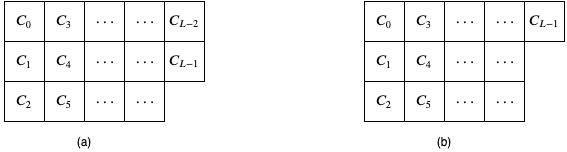
\includegraphics[width=\textwidth]{cosetRep.jpg}
		\caption{Turbo Encoder}
		\label{fig1}
		\end{figure}
		
Figure \ref{fig1} (a) represents the case where $L \mod \tau =2$ and Figure \ref{fig1} (b) represents the case where $L \mod \tau =1$. The task is to generate a permutation matrix which guarantees that the should a weight-$2$ RTZ $x^t(1+x^3)$ occur it will not be mapped to the same RTZ sequence at all points during interleaving.

The $L \times N$ permutation matrices which meet the criteria are shown in Table \ref{tb4} for different values of $L$ and $N$. 

 \begin{table}[h!]
\centering
\begin{tabular}{|c || c  c  c  c  c  c c|} 
 \hline
 $L=4,N=12$ & 0 & 3 & 6 & 10 & & &\\ 
  \hline
 $L=5,N=15$ & 0 & 3 & 6 & 10 & 12 & &\\ 
  \hline
\end{tabular}
\caption{All unique permutation matrices for different values of $N$ and $L$ when $L \mod \tau =1$ or $L \mod \tau =2$}
\label{tb4}
\end{table}

%Permutation matrices are usually square in nature. Representing a permutation matrix in Table \ref{tb4} by $\mathbf{A}$ we form the required $N \times N$ permutation matrix, by concatenatenating 3 permutation matrices and circularly shift each consecutive matrix by $\tau-1$ to right as shown in Equation \ref{eq1}.

The permutation matrices obtained using this method ensures that weight-$2$ RTZ $x^t(1+x^3)$ is never mapped to itself at any point in the interleaving process.

 \section{Weight-$3$ RTZ inputs}
 In most interleaver design cases, focusing on weight-2 RTZ inputs would be enough. For the $5/7$ RSC interleaver however, this is not the case since the minimum weight codeword is caused by the weight -$3$ RTZ input of the form $x^t(1+x+x^2),~t=1,2,...$.  In general, any time a weight $3$ input has $x \mod 3=1$ zeros and/or $x \mod 3=1$ between its first 2 ``1'' bits and and last 2 ``1'' bits it is a weight $3$ RTZ input sequence. This definition is specific to the $5/7$ RSC encoder. 
 
 Similar to the approach taken for designing interleavers weight-$2$ RTZ sequences, we group the interleavers into 3 groups, depending on the value of $L \mod \tau$ and find all possible permutation matrices which prevent $x^t(1+x+x^2)$ from being mapped to itself.
 
 \subsection{Interleavers with coset length $L$ where $L \mod \tau =0$}
 Table \ref{tb5} list all permutation matrices when which transforms $x^t(1+x+x^2)$ into a non RTZ input.
 
\begin{table}[h!]
\centering
\begin{tabular}{|c || c  c  c  c  c  c  c  c  c |} 
 \hline
 $\mathbf{A}$ & 0 & 3 & 6 & 1 & 4 & 7 & 2 & 5 & 8\\ 
  \hline
 $\mathbf{B}$ & 0 & 3 & 6 & 1 & 4 & 2 & 7 & 5 & 8\\ 
 \hline
$\mathbf{C}$ & 0 & 3 & 6 & 1 & 4 & 2 & 8 & 7 & 8\\ 
 \hline
$\mathbf{D}$ & 0 & 3 & 6 & 1 & 4 & 2 & 5 & 8 & 7\\ 
 \hline
 $\mathbf{E}$ & 0 & 3 & 6 & 2 & 5 & 1 & 4 & 7 & 8\\ 
 \hline
 $\mathbf{F}$ & 0 & 3 & 6 & 2 & 5 & 1 & 4 & 8 & 7\\ 
 \hline
 $\mathbf{G}$ & 0 & 3 & 6 & 2 & 5 & 1 & 8 & 4 & 7\\ 
 \hline
  $\mathbf{H}$ & 0 & 3 & 1 & 6 & 4 & 7 & 2 & 5 & 8\\ 
 \hline
  $\mathbf{I}$ & 0 & 3 & 1 & 4 & 7 & 2 & 5 & 6 & 8\\ 
 \hline
 $\mathbf{J}$ & 0 & 3 & 2 & 6 & 5 & 8 & 1 & 4 & 7\\ 
 \hline
  $\mathbf{K}$ & 0 & 3 & 2 & 5 & 8 & 1 & 4 & 6 & 7\\ 
 \hline
  $\mathbf{L}$ & 0 & 1 & 3 & 4 & 7 & 2 & 5 & 6 & 8\\ 
 \hline
\end{tabular}
\caption{All unique permutation matrices for the case when $L \mod \tau =0$}
\label{tb5}
\end{table}
 
 However, there are other weight 3 RTZ inputs which exist within this span, depending on the permutation matrix that is chosen. For example, $\mathbf{A}$ has  $1 +x^4+x^8,~ 1+x^5+x^7, ~x+x^3+x^8,~ x+x^5+x^6,~x^2+x^4+x^6,~x^2+x^3+x^7$, whiles $\mathbf{B}$ has $1+x^4+x^8,~x+x^3+x^8,~x+x^3+x^5,~x+x^6+x^8,~x^2+x^3+x^7,
 ~x^2+x^6+x^7$
 
 Regardless of which permutation matrix is picked, we are certain that the weight 3 RTZ $1+x+x^2$ will not be mapped to itself within the chosen span.
 
 \subsection{Interleavers with coset length $L$ where $L \mod \tau =1$ or $L \mod \tau =2$}
 
Similar to weight 2 RTZ, we further divide the abpve case into 2 categories. The first category is when $N$ is divisible by $3$ and $6$. The second category is where $N $ is divisible by 3 only. Table \ref{tb6} show all permutation matrices which prevent $1+x+x^2$ from being interleaved to itself when $L \mod \tau =1$ or $L \mod \tau =2$ and $N$ is divisible by $3$ and $6$.
 
 \begin{table}[h!]
\centering
\begin{tabular}{|c || c  c  c  c  c  c |} 
 \hline
 $\mathbf{A}$ & 0 & 3 & 1 & 4 & 2 & 5\\ 
  \hline
 $\mathbf{B}$ & 0 & 3 & 2 & 5 & 1 & 4\\ 
 \hline
\end{tabular}
\caption{All unique permutation matrices for the case when $L \mod \tau =1$}
\label{tb6}
\end{table}
 
 The remaining weight 3 RTZ which need to be dealt with is $1+x^2+x^4$. 
 
 
 For the second category ($N$ divisible by $3$ only), there are no permutation matrices which meet this criteria.
 
  \subsection{Alternate Method for Interleavers with coset length $L$ where $L \mod \tau =1$ or $L \mod \tau =2$}
  For the case where  $L \mod \tau =1$, there is a point where $1+x+x^2$ is mapped to itself, depending on $N$.
  
  For the case where  $L \mod \tau =2$, $1+x+x^2$ is never mapped unto itself, but the lowest weight $3$ RTZ that needs to be dealt with is $x+x^3+x^5$
  
  \section{Maximizing Seperation for weight-2 RTZ inputs}
  
 \subsection{case $L \mod 3 =0$}
  From Table \ref{tb1} we select the permutation matrix $\mathbf{A}$. For interleaver length $N>9$, we repeat this pattern. With this permutation matrix, we are sure that the weight-2 RTZ $1+x^9$ will be mapped to itself. We wish to prevent this by transforming $1+x^9$ into a weight -2 RTZ input which has a large seperation the ``1'' bits. Let $t$ and $s$ represent the seperation before and after interleaving.It is worth noting that $t,s$ are multiples of $\tau =3$
  
  The mamimum seperation depends on the value of N. Therefore to achieve the largest separation after interleaving $s$ must meet the following condition. 
  
   $$s=\text{max} \begin{cases}
       a\leq\lfloor\frac{N}{2}\rfloor 
    \end{cases}
$$

\subsection{case $L \mod 3 =1$}

\subsection{case $L \mod 3 =2$}
\section{Maximizing seperation for weight-$3$ RTZ inputs}

\subsection{case $L \mod 3 =0$}

\subsection{case $L \mod 3 =1$}

\subsection{case $L \mod 3 =2$}

\section{Maximizing Seperation for weight-$2$  and weight-$3$ RTZ inputs}

\subsection{Choice of Permutation polynomial}
\paragraph{case $L \mod 3 =0$}

\paragraph{case $L \mod 3 =1$}

\paragraph{case $L \mod 3 =2$}

\subsection{Range of Maximum Separation}

\section{Interleaver implementation}

\section{Simulation Results}
 \end{document}
